\label{sec:3_methodology}

\begin{comment}
This chapter may have many names. Lately, many have named it “Methodology”, but names like “Design and Implementation”, a “name” of a developed system, etc. are also often used. Just find a name that matches your research. Regardless, the important thing here is to describe YOUR research.

INTRO: Again, start the chapter with a sentence or two explaining why you have this chapter (repeating the last sentences from the proposed summary in the previous chapter) - assuming that some readers have not read the previous chapter.

MIDDLE SECTIONS: What are your ideas? Your solutions. How have you done “things”? Implementation details. Frameworks used. Etc. Also, discuss alternative ways of doing things and explain why you have chosen to do things as you have. WHAT! HOW! WHY!

SUMMARY: End this chapter with a summary section. Summarize what you have done and why! Main knowledge gained. What have we learned? Lead to the next chapter, stating that you will test your prototype.
\end{comment}


% INTRO:


% MIDDLE SECTIONS:
    % Implementation
    \section{FLEX-VQA}
    \label{sec3:flex_vqa}
        \subsection{Overview}
        % What:

        % FLEX
        Two ways to address this task are to make \gls{vqa} methods more transparent and explainable. Since the task has two modalities, namely vision and language, the explanation can come from either the language model, the image model, or both. This thesis will address this task using the cross-modality explanation method \gls{flex} proposed by Wickramanayake et al. \cite{wickramanayakeFLEXFaithfulLinguistic2019}. An overview of the \gls{flex} model has been described shortly in sub-chapter \ref{sec:2_related_work} on page \pageref{sec:2_related_work}. This method is relevant for this thesis because it takes the explanation task to the network's visual module and can explain why a picture should be in a given class using natural language. It combines a \gls{cnn} pretrained on the given task and does not need any training that modifies this pretrained image model when training to give explanations. An overview of the \gls{flex} framework can be seen in Figure \ref{fig:flex_overview}.

        \begin{figure}[htb]
            \centering
            \centerline{
            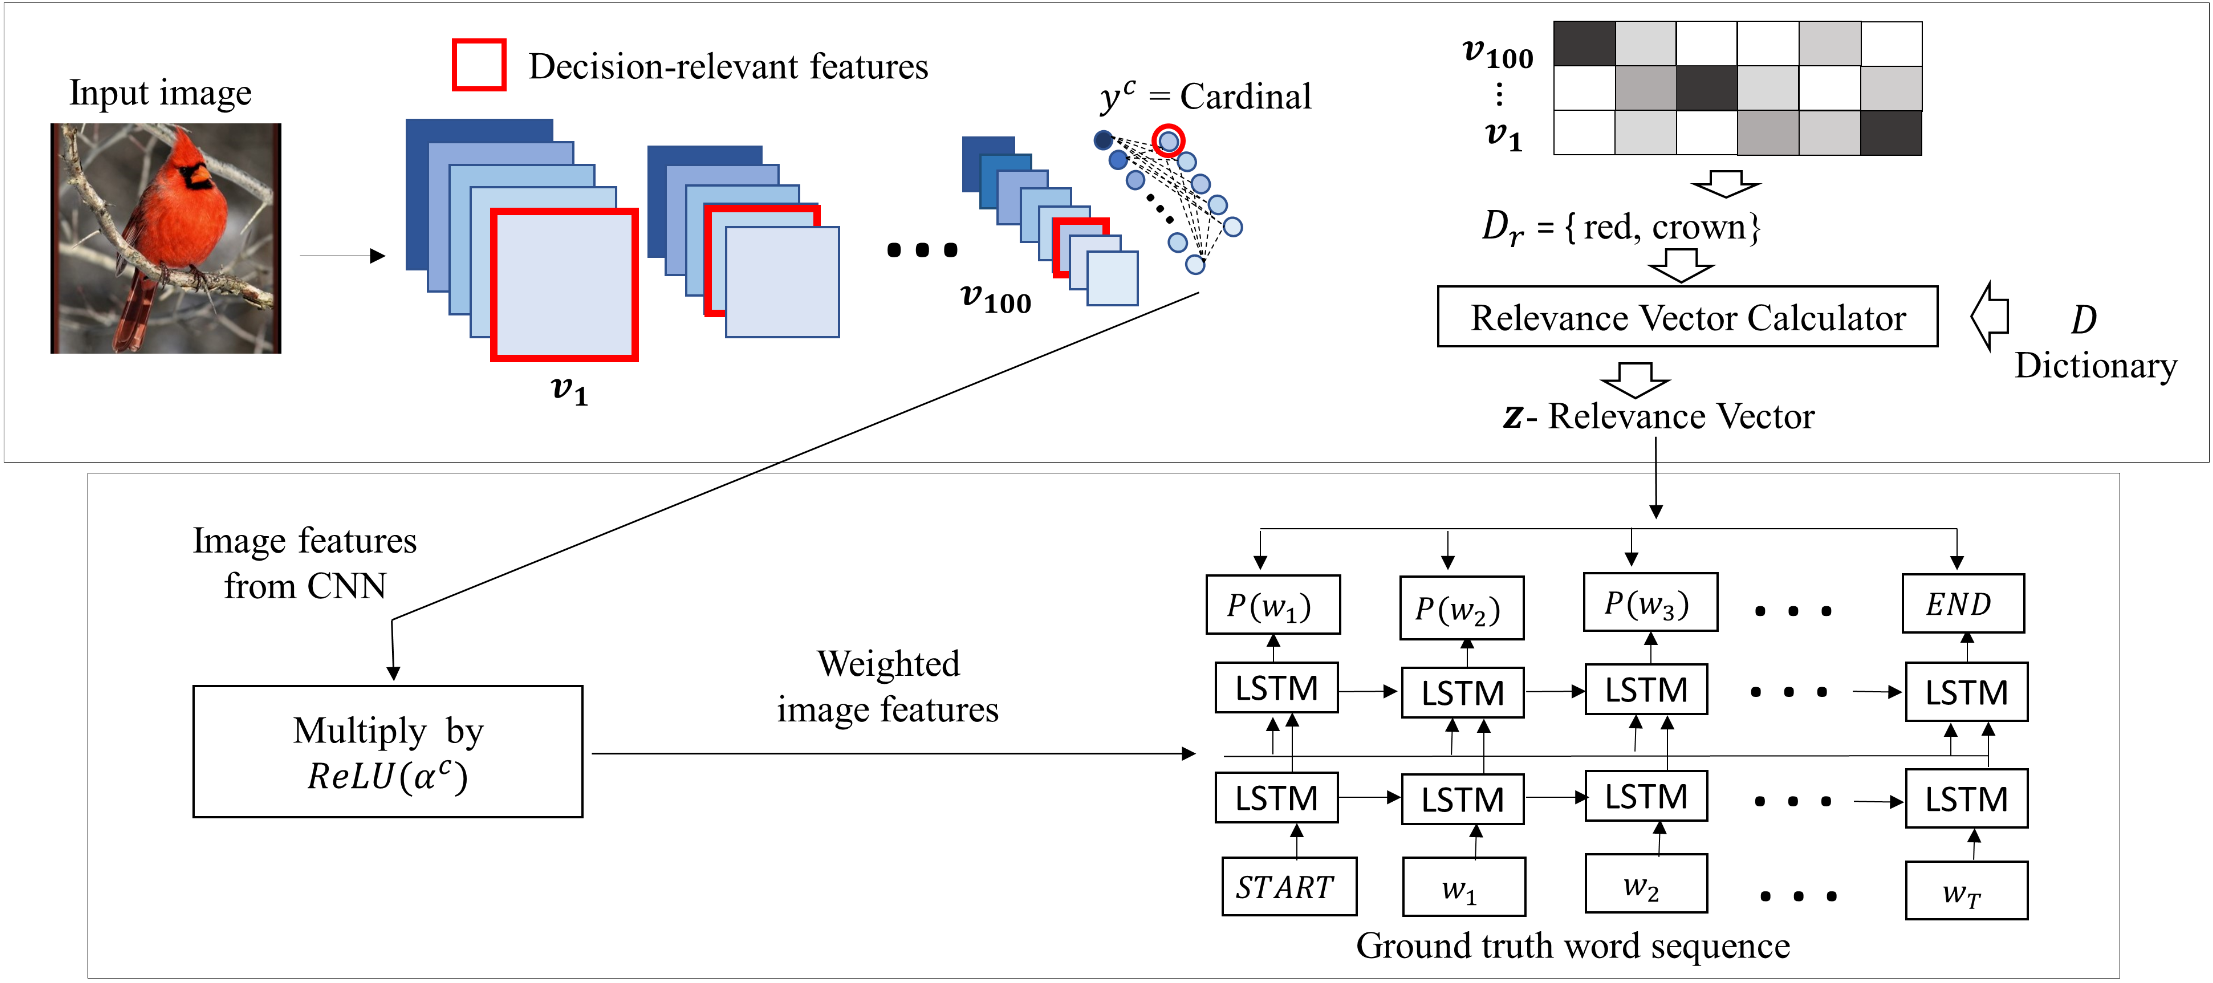
\includegraphics[width=17cm]{images/FLEX_overview.png}}
            \caption{Overview of the FLEX Framework.\\
            Figure credit: Wickramanayake et al. \cite{wickramanayakeFLEXFaithfulLinguistic2019}.}
            \label{fig:flex_overview}
        \end{figure}

        % More in detail on how FLEX works. 
        Given an image and its predicted class $c$, the method finds a subset of the most important feature maps from each layer in the pretrained \gls{cnn}. To find the global activation score of each layer, it sums up each neuron in the layer, gives this score as an activation score, and then repeats for every layer. Thereafter it sorts the layers in order of importance and chooses a subset of $n$ layers so that the subset has combined importance over a chosen threshold. When a subset of the most important visual features is collected, \gls{flex} connects these visual features with linguistic features. The goal of using \gls{flex} is to find a connection score between a word ($w$) to every important element in the subset of feature maps ($F$) so that the word ($w$) best describes the important visual element ($v$) in each feature map. With a given ground truth description ($D_I$) of an image ($I$) in natural language, \gls{flex} uses this description for every image and builds a dictionary that contains all words in every description. This dictionary is called ($D$) and is used when describing new images that do not have a ground truth description. For each word ($w$) \gls{flex} calculates co-occurrence score for each feature ($v \in F$), using the Dice score \cite{diceMeasuresAmountEcologic1945, sorensenMethodEstablishingGroups1948}. The word with the highest co-occurrence score gets associated with the visual feature ($v$). 



   
        This labeling of visual features can be reminiscent of DenseCap proposed by Johnson et al. \cite{johnsonDenseCapFullyConvolutional2016}, and Neural Baby Talk proposed by Lu et al. \cite{luNeuralBabyTalk2018}. The main difference between these methods and \gls{flex} is that \gls{flex} can be added to a network after the architecture is finalized, trained, and evaluated. In theory, it is agnostic to the underlying network as long as the visual encoder has a property that allows it to find different parts of the network that correspond to different parts of an input image. \gls{flex} uses the \gls{gradcam} technique proposed by Selvaraju et al. \cite{selvarajuGradCAMVisualExplanations2020} to do a backward pass through the feature maps of the \gls{cnn} to find the largest class activation maps when predicting a class. This information is then used to map words to important visual feature extractions in the network. This mapping of words combines the separable feature layers salient layers of the \gls{gradcam} method with natural language to make better explanations.


        \subsection{Implementation}
        % How:
        Given that \gls{flex} can combine information from the visual domain with natural language, it is an exciting framework to explore in the field of \gls{xai} and \gls{vqa}. A modified architecture to \gls{flex} is presented in this thesis, as seen in Figure \ref{fig:architecture_proposal}. This proposed architecture has unfortunately not been tested in this thesis because of technical hurdles outside the scope of this thesis. A more detailed explanation of these hurdles can be seen in subsection \ref{subsec:no_flex}. However, since a lot of the available time for this thesis was put into researching this approach and finding the technical hurdles until deciding that solving these hurdles was not relevant to this thesis, an overview of the architecture will still be proposed. 

       

        % Input from essay here.
        \subsection{Proposed architecture}
        \label{sec3:proposed_architecture}
        
        Figure \ref{fig:architecture_proposal} shows how the data flow in the proposed method can work. It closely follows the \gls{flex} \cite{wickramanayakeFLEXFaithfulLinguistic2019} architecture proposed by Wickramanayake et al. It consists of a \gls{cnn} that extracts visual information and a 2-layered \gls{lstm} \cite{hochreiterLongShorttermMemory1997} \gls{rnn} that combine linguistic information with extracted visual features. This architecture is relevant for this thesis because it uses a backward pass to find locally accurate visual features, which are then used to give an image caption that describes what visual features were important to the classification and captioning of the image. This makes the architecture valuable as a starting point for this thesis and can be adapted to use \gls{vqa} datasets as linguistic input to make it possible to ask questions regarding the classification of images and predictions. 
        
        % Explain the proposed data flow/architecture 
            % Training
            % CNN
        During training, the proposed architecture takes an image and its corresponding questions and answers from the \gls{vqa} dataset. The images are fed through a \gls{cnn}-network, which can be pretrained on a larger dataset, like ImageNet \cite{dengImageNetLargeScaleHierarchical2009}. This is because the explaining method utilizes feature maps in each layer of the \gls{cnn}, so it is agnostic on what type of \gls{cnn} it is and what dataset it is trained on earlier. The \gls{cnn} predicts a class of what it sees in the image and, with a backward pass, finds important feature maps in each  convolutional layer. Each feature in the set of important feature maps gets associated with a word and stored in a relevance vector. This process is done by computing a co-occurrence score between each word in the ground truth caption and the feature. The feature with the highest co-occurrence score gets linked with that feature. 
        
            % LSTM
        The \glspl{lstm} gets trained by feeding each word in the ground truth caption into the first layer alongside the hidden state of the \gls{lstm}. This is used to compute the next state, which gets concatenated with important visual features and is input to the second and last, \gls{lstm}-layer. 
        The output from the second \gls{lstm}-layer is encoded to vocabulary space that is used to make a conditional probability distribution that later will be used to calculate the probability for predicting that word, given the given image features. 
        
            % Testing
        The architecture takes an image and an optional question as input during prediction. The \gls{cnn} extracts important features in the layers, which get fed into the \gls{lstm}. Important feature maps from the \gls{cnn} are also used to calculate the relevance vector between features in the image and words. The \gls{lstm} uses this relevance vector alongside important decision-relevant features from the image to predict a word. This word prediction is repeated until the stop word is predicted. 
        
        If no question is input to the algorithm during prediction, the model will use the most accurate predicted answer caption that describes the image as a whole as a caption for the image. On the other hand, if a question is submitted alongside the image, the \gls{lstm} will generate captions that answer the question asked and then chose the most decision-relevant answer as the caption. 
        
        
        
        % Data flow
        \begin{figure}[htb]
            \centering
            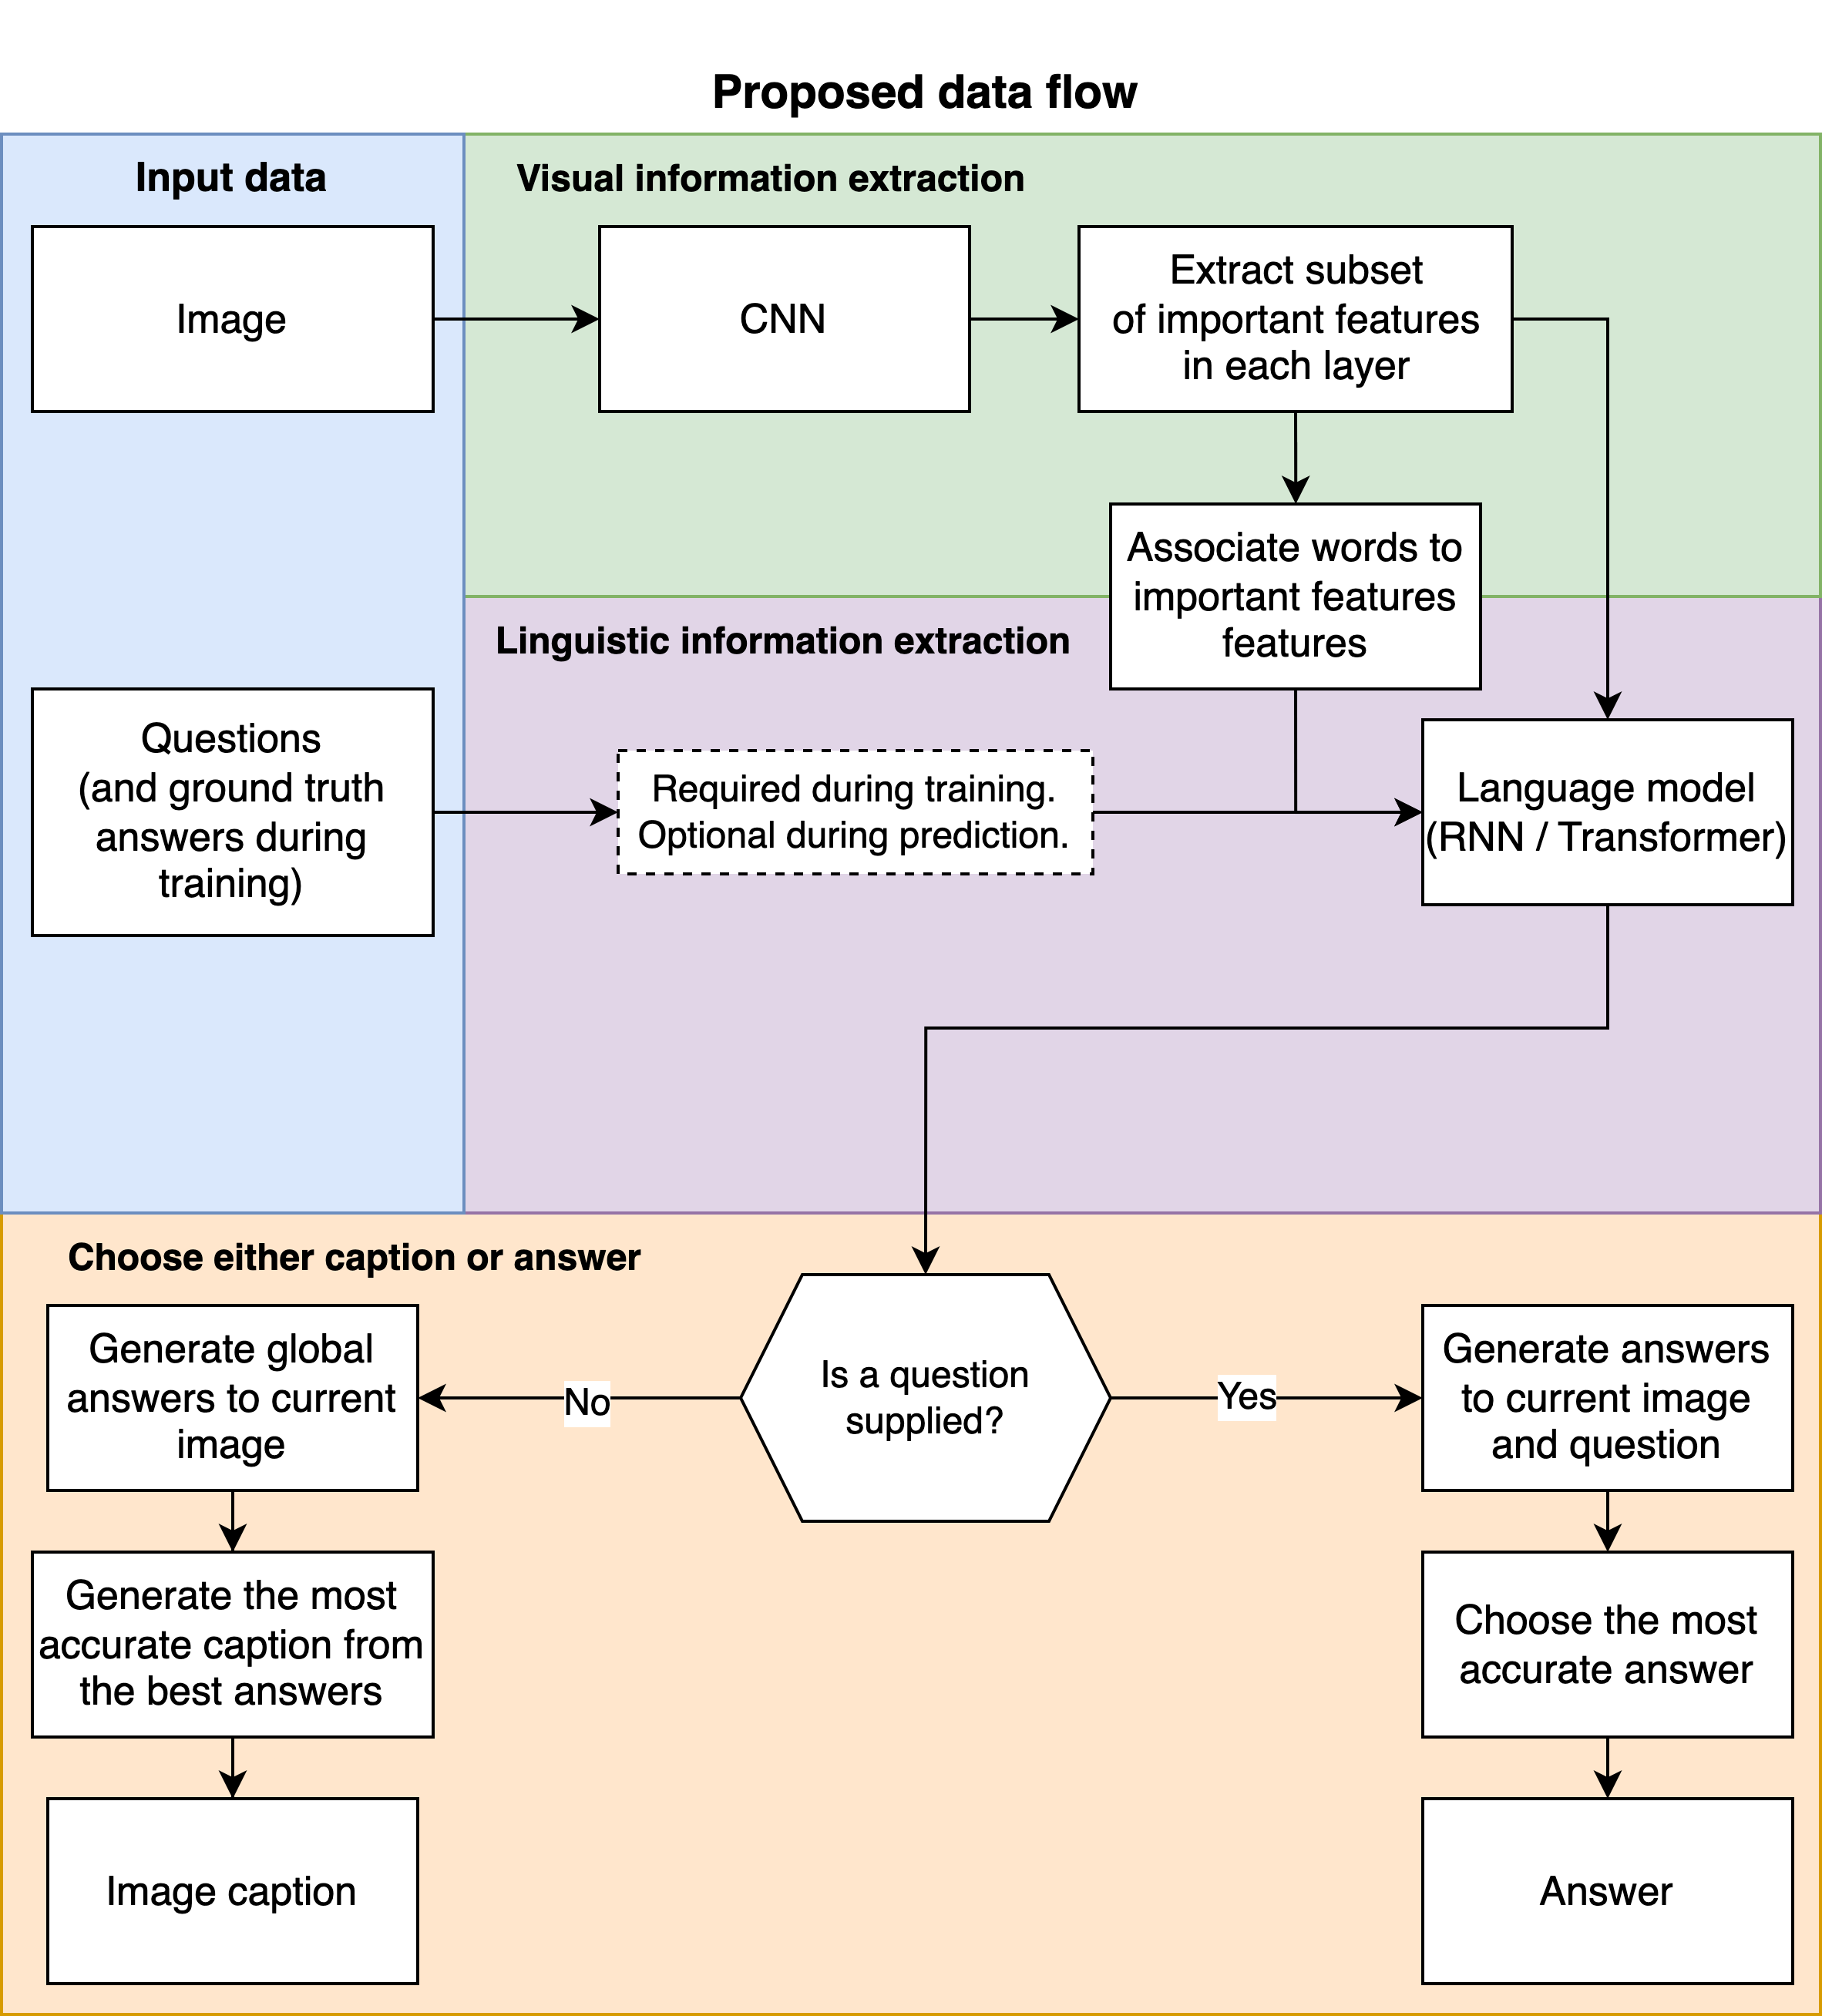
\includegraphics[width=\linewidth]{images/architecture_proposal.png}
            \caption{Proposal of the data flow and components that will be explored in this thesis.\\
            Figure by the author.
            }
            \label{fig:architecture_proposal}
        \end{figure}
                
                
        

        % Why:

        By using \gls{flex} as a starting point, this thesis wants to explore how to make it able to be used for explainable \gls{vqa}. To adapt the \gls{flex} framework to \gls{vqa}, the dataflow shown in Figure \ref{fig:architecture_proposal} is proposed. Using this technique, a user can get an answer for a question regarding an input image that is both in natural language, faithful to the underlying \gls{cnn} model, and explainable. The explanation is faithful to the underlying model since it uses the actual gradients in the \gls{cnn} to find the words used in answering the question. This feature guarantees that if the underlying \gls{cnn} model has learned features that correlate with the answer but are not the intended or logical features to pay attention to, these flaws get communicated to the user in natural language. Making a model that is able to explain what it weighs as important to a user, also when flawed, is important in making a system that a user can make a factually based decision in trusting or not. 

        Neither the \gls{cnn} nor the \glspl{lstm} needs to be specifically trained to be explainable. The architecture uses the underlying nature of the models to build an answer that is transparent to the underlying model and explains to the user what the model values as important. 



        \subsection{Why this method has no experiments}
        \label{subsec:no_flex}

            % Intro
            To implement the proposed architecture, as shown in Figure \ref{fig:architecture_proposal}, using the original code from the \gls{flex} paper as a starting point was natural.
            The authors of the \gls{flex} paper also released the code used to do the experiments in the article. The experiments use an \gls{cnn} called Compact-Bilinear Pooling, which is a classifier proposed by Gao et al. \cite{gaoCompactBilinearPooling2016}. While the FLEX framework is designed to be model agnostic, the actual implementation of the experiments is tied closely with the \gls{cnn}, which has proven to be a hurdle when trying to both recreate the results in the paper and expand on the architecture and features. The main reason why this method has no complete experiments or results is an outdated machine learning framework.
    
            
            \paragraph{The original implementation of FLEX\\}
            \gls{flex} need to be able to name feature maps in a given \gls{cnn}. This is an essential part of the framework and therefore needs to have insight into how the layers of the \gls{cnn} are structured.
            The implemented version of the original \gls{flex} architecture uses the Compact-Bilinear Pooling \gls{cnn}, which in short, uses kernelization to reduce the number of dimensions of bilinear features to make it more computationally efficient at the cost of having an architecture that deviates somewhat from the traditional \gls{cnn} architecture. The authors of the \gls{flex} paper, therefore, have implemented a version of the framework that addresses these special considerations when calculating co-occurrence metrics between words and features. 
        

            \paragraph{Why Caffe was needed\\}
            % Why Caffe was needed
            To use the same \gls{cnn} in a new context, as in this thesis, would require retraining or fine-tuning this network to suit the images in the given dataset. This would require the Compact-Bilinear Pooling model to train or choose a new \gls{cnn} that could be merged with the \gls{flex} framework. The original Compact-Bilinear Pooling came with pretrained weights from training on the Caltech-UCSD Birds (CUB) \cite{PeronaLabCUB2002011} dataset. This dataset has images from Flickr and ImageNet but is solely focused on bird species and a rather small amount of images (11,788, compared to 14 million images in ImageNet \cite{dengImageNetLargeScaleHierarchical2009}). Therefore the original weights are best to classify this exact dataset but require retraining outside of this specific task.

            \paragraph{Getting Caffe to run\\}
            % Getting Caffe to run
            To get Compact-Bilinear Pooling to train on a new dataset, the underlying machine learning framework it was built in had to be installed. This framework is named Caffe and is a deep learning framework developed by Berkeley AI Research (BAIR) / The Berkeley Vision and Learning Center (BVLC) and is a precursor to Caffe2, which was originally built by Facebook and merged with PyTorch. This forking and merging of newer versions of the Caffe framework have stagnated the development of the original Caffe framework, which has not received an update since 2017. The \gls{flex} framework is implemented in TensorFlow version 1.7, which is considered legacy at the time of writing. Because of the rapidly evolving nature of both software and hardware since 2017, it proved to be a nontrivial task to get Compact-Bilinear Pooling written in Caffe to run on the available hardware.

            To run the Caffe framework on \glspl{gpu}, to get the compute benefits necessary for deep learning, the framework supports \glspl{gpu} from Nvidia with \gls{cuda} version 5 through 8 \cite{CaffeInstallation, CaffeDeepLearning} and AMD \glspl{gpu}. The \glspl{gpu} in the compute cluster available to run experiments for this thesis are Nvidia RTX 2080 Ti, Nvidia A100, and AMD Vega 10 XL/XT, which run \gls{cuda} version 11.7, 11.5 and ROCm version 4.5.0 respectively \cite{MLNodesUniversitetet}. To not break compatibility with other services on the compute cluster, containerization was needed. Luckily containers are being actively deployed for Caffe with \gls{gpu} support, most notably from Nvidia and AMD.

            At the time of starting implementing the architecture described in Figure \ref{fig:architecture_proposal}, communication with the IT staff at the University of Oslo, responsible for the compute cluster available, was established. At that stage, only an experimental stage of containerization was available through the container engine Podman \cite{Podman}. Using this container engine, the Nvidia container could not attach the Nvidia \glspl{gpu}. However, the AMD ROCm container could access the AMD \glspl{gpu} but did not have the correct driver compatibility to train the \gls{cnn}. Since Podman did not result in a container that could run successfully, a different container engine was installed, namely Apptainer, formerly known as Singularity. This new engine was able to see all the Nvidia \glspl{gpu}, but not the AMD ones. After the initial errors were ironed out, a Caffe container from Nvidia was successfully installed. Although successfully installed, the container had trouble running the training examples in the \gls{flex} code repository. While not a definite problem could be addressed because there were several different error messages. When the current error message was solved, a new one arose. The most likely explanation for the error messages was an incompatibility issue between the Caffe version in the container and the hardware it was tested on. After extensive testing and error-solving in seven months, the decision was taken that this technical problem was outside this thesis's scope, and this method was discontinued for this project. 
            

            
            \paragraph{How these problems could have been mitigated\\}
            % How this could be fixed.
            % implemented from scratch. 

            There are still some ways this method could be implemented. The main limitation of the chosen approach was to get the Caffe framework up and running, but there are still interesting ways to run experiments with the proposed method. Some proposed improvements based on the experience gained implementing this method are:

            \begin{itemize}
                \item \textbf{Remove Caffe from FLEX\\} 
                To have better compatibility with modern hardware and be more accessible to research moving forward, discontinued frameworks should be updated with more up-to-date versions. At the time of publishing the FLEX paper (2019), the development of the Caffe framework had already been stale for two years. To make research easier to peer-review and implement by others so that the proposed method can be further built upon, all researchers are served with publishing material that others can follow and implement themselves. By removing the Caffe framework from the FLEX framework, the method gets more accessible and easier to expand by others.
                

                \item \textbf{Update FLEX to TensorFlow 2\\}
                The FLEX framework is implemented in TensorFlow version 1.7, which was released in 2018. As of writing this thesis, TensorFlow versions 1.x are considered legacy. However, version 1.15, the latest version 1.x, is supported by TensorFlow 2. By updating to a more recent version, the framework can implement more modern features, gain compatibility with modern hardware and gain more users familiar with the current versions. This upgrade can both speed up the implemented FLEX framework through software and hardware optimizations, as well as speed up the development of the framework itself. 
                TensorFlow has migration guides and scripts to help translate from version 1 to 2 \cite{MigrateTensorFlowTensorFlow}, which makes the migration manageable. 
    

                \item \textbf{Make FLEX model agnostic in practice\\}
                In theory, the \gls{flex} framework is separate from the \gls{cnn}. As proposed in the published paper, the implemented FLEX framework would benefit from being adapted to be agnostic to the underlying method. The originally implemented method has modified methods to extract image features from the specific \gls{cnn}. By using an agnostic implementation of the gradient search through the \gls{cnn} feature maps, the method could be expanded upon by allowing to test of different \glspl{cnn} to extract features and find co-occurrences with linguistic features. This could make the method more straightforward to implement for new \glspl{cnn}, which could make new methods more explainable.

            \end{itemize}

        % Outro / summary
        \subsection{Summary of FLEX-VQA}
        To summarize, by implementing the \gls{flex} framework into a \gls{vqa} method, the combined framework would make interpreting \gls{vqa} models easier and locally accurate. \gls{flex} has on a overall lever the same benefits as \gls{lime}, of being locally accurate. By having insight into a locally accurate explanation model, the method would make it possible for both researchers and users of an implemented system to see if the underlying model is trustworthy based on what the model deems important. 




    \section{Alpaca-VQA}
    \label{sec3:alpaca_vqa}

        \subsection{Overview}
        % What:
        To make a \gls{llm} that can see the world and explain what it sees, it was outside the scope of this thesis to train a model from scratch, both regarding time and resources. A \gls{llm} requires vast amounts of data when training, not only a large amount but also that it has good quality. Training the model requires large compute clusters that consume lots of energy, cost much to facilitate, and produce greenhouse emissions \cite{??}. Therefore, a \gls{llm} that was already pretrained was needed for this thesis to be fine-tuned further to answer the research goals. 

        


        % Alpaca-LoRA
        Even though the Stanford Alpaca model was trained using significantly less computing power compared to other \glspl{llm}, it is still advantageous to further lower the necessary compute budget to train and fine-tune models. A technique that was proposed by Hu et al. called \gls{lora} \cite{huLoRALowRankAdaptation2021} addresses this issue. The way they address this task is to add pairs of rank-decomposition weight matrices, commonly referred to as update matrices, on the existing weights and only train these newly added weights. This has many advantages, most importantly accelerating the training while reducing memory consumption. Other advantages of these added matrices are that the original weights are kept frozen, making the \gls{lora} model less prone to catastrophic forgetting. The added weights are also typically less than 10 percent of the original trainable parameters, making it more feasible and faster to train domain-specific models that can change the smaller \gls{lora} weight matrices on the fly to more accurately answer a task. When using \gls{lora} matrices, they also allow both training and interference on consumer hardware, like desktop \glspl{gpu} and even single-board computers like Raspberry Pi's \cite{artemandreenko[@miolini]VeSucefullyRunned2023}. 


        \subsection{Implementation}
        % What I did implement
        To address the research questions stated in \ref{sec:1_2_problem_statement}, considering ??, a \gls{lora} version of the Stanford Alpaca version was used to carry out the experiments. The code used as a starting point is a fork of Erik J. Wang's Alpaca-LoRA \cite{wangAlpacaLoRA2023}, which was further modified to fit this thesis' experiments. The most notable modification to this model is to make it cross-modal by allowing it to take both text and images as input.

        \subsubsection{Make a language model see images}
        % How to get the model to see
        An image encoder had to be implemented to make the model able to interpret images. To make the \gls{llm} able to do the interpretation of image data, the visual features had to be extracted in a manner that allowed it to be fused with the text input. Also, to make it more efficient to experiment with different image encoders, a dataflow that first finds an image-to-text feature that is incorporated into the text input prompt to the language model. In Figure \ref{fig:alpaca_vision}, the proposed dataflow is shown. This architecture allows the language model to be agnostic to the image encoder, which allows it to use a fine-tuned \gls{cnn} or vision transformer for a specific task. 

        % Data flow
        \begin{figure}[htb]
            \centerline{
            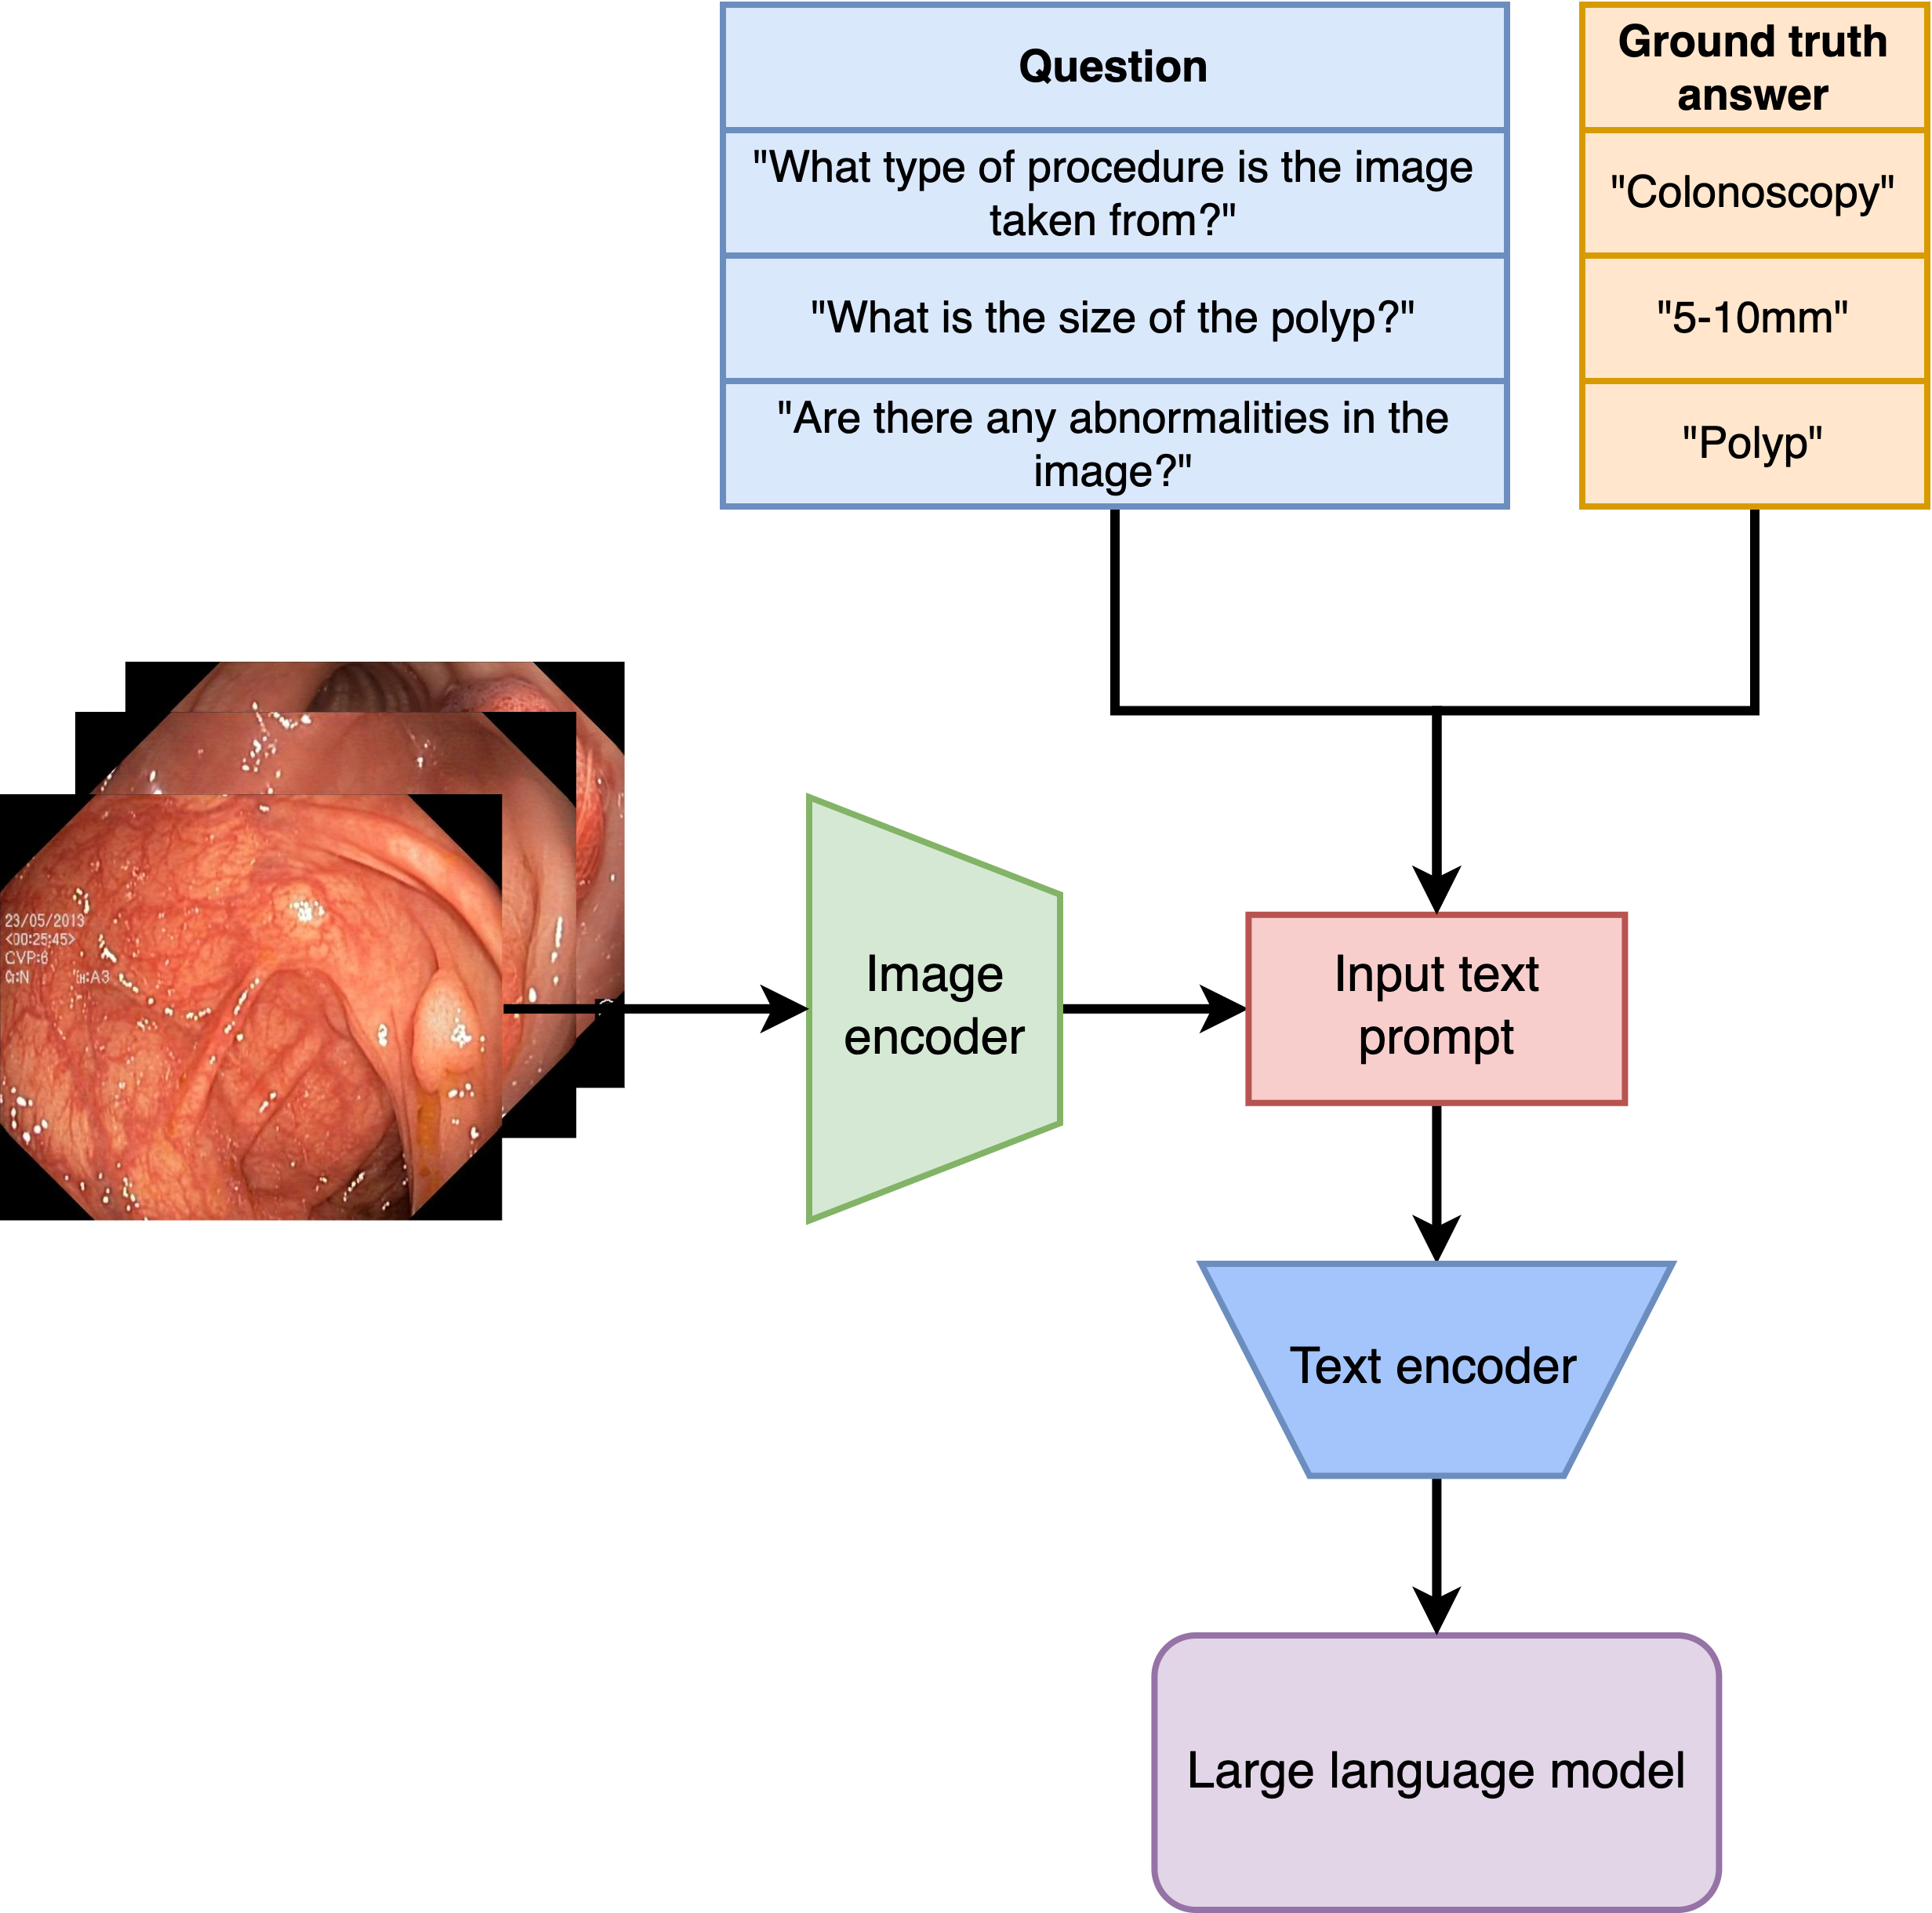
\includegraphics[width=\textwidth]{images/alpaca_vision.png}}
            \caption[Overview of the proposed dataflow to make large language models interpret images.]{Overview of the proposed dataflow to make large language models interpret images. The images represented in this Figure are from the HyperKvasir dataset by Borgli et al. \cite{borgliHyperKvasirComprehensiveMulticlass2020}. The rest of the diagram is by the author of this work.}
            \label{fig:alpaca_vision}
        \end{figure}


        % How & Why :
        Specifically, the image encoder first implemented was \gls{vgg}-16, proposed by Simonyan and Zisserman at Oxford \cite{simonyanVeryDeepConvolutional2015}. The rationale for implementing this \gls{cnn} first is that it’s a well-known network that achieves relatively good performance on the ImageNet dataset, with 92.7\% on the test set. The VGG-16 model used for the initial experiments is pre-trained on the ImageNet \cite{dengImageNetLargeScaleHierarchical2009} dataset. The model would most presumably perform better if pretrained on the specific dataset used, namely the HyperKvasir dataset \cite{borgliHyperKvasirComprehensiveMulticlass2020} made by Borgli et al. However, the initial experiments will explore the proposed approach's feasibility rather than achieve optimal accuracy.

        % Explain why VGG-16 should work even if it does not give regions of interest
        Given that the VGG-16 network is pre-trained on ImageNet, it outputs a probability for each of the 1000 classes in the dataset. To address the task of extracting features from any image, regardless of if the \gls{cnn} is pretrained on the task, the method implemented extracts the top 100 ImageNet highest probability classes. With this approach, the image feature extraction will find a consistent amount of features in an image, sorted with the feature with the highest probability first. The features with the highest probability are the features most likely to have a feature map similar to a class in ImageNet. Therefore, even if the class label from ImageNet is not connected with a correct label from the HyperKvasir dataset, there is a high probability that the feature extraction will still be useful to extract image features. 

        The VGG-16 \gls{cnn} was originally developed for the image classification task, not object classification. It consists of multiple convolutional layers followed by fully connected layers, and it does not have any built-in mechanisms for handling \gls{roi} operations. Consequently, VGG-16 only is made to be an image classifier and only outputs classes it detects in the image as a whole. Object classifiers, like R-CNN \cite{girshickRichFeatureHierarchies2014}, Faster R-CNN \cite{renFasterRCNNRealTime2015}, and variants of YOLO \cite{redmonYouOnlyLook2016, redmonYOLO9000BetterFaster2016, redmonYOLOv3IncrementalImprovement2018, bochkovskiyYOLOv4OptimalSpeed2020, jocherYolov5, liYOLOv6SingleStageObject2022, wangYOLOv7TrainableBagoffreebies2022, jocherYOLOUltralytics2023}, among others are also made to output \gls{roi}, which would allow the image encoder also to encode locations of a detected object within the image. These object classifying qualities from an image encoder will most likely give the \gls{llm} more and more accurate data to work from. However, the initial experiments will test the feasibility of the implementation using VGG-16. When the feasibility of this method is confirmed, other image encoders will be tested and compared to the VGG-16 version.

        % More info on the other image encoder


        \paragraph{Images to text prompt\\}
        % How to encode images into text
        In order to encode the image features into a format that \gls{llm} can interpret, the image features must be converted into a format that can be embedded in a natural language question-and-answer format. The dataset used to train the Stanford Alpaca model follows a question-input-answer format, as shown in Figure \ref{fig:alpaca_prompt_format}. To make the new task of interpreting images and keeping the prompt text format as close to the original, image features ought to be incorporated into the input section of the original prompt better to utilize the already pre-trained structure of the model. The feasibility of incorporating image features in text prompts has been successfully explored by Yang et al. in the paper MM-REACT \cite{yangMMREACTPromptingChatGPT2023}. The team explores methods to make ChatGPT multimodal reasoning and action, including interpreting images. 
        
        They achieve this by using an image encoder, proposed by Zou et al. \cite{zouGeneralizedDecodingPixel2022}, with \gls{roi} capabilities using dense captioning, which outputs class labels and coordinates of the corners of bounding boxes. These extracted features are then concatenated into a text string that the \gls{llm} receives as an input prompt. The modified Alpaca model used in this thesis uses a similar approach to the one in MM-REACT but is adjusted to use the features received by the tested image encoder. When the VGG-16 model is used, the final text prompt to the Alpaca-LoRA model is the same as shown in Figure \ref{fig:alpaca_modified_prompt_format}.
        
        % Original prompt format
        \begin{figure}[htb]
            \centerline{
            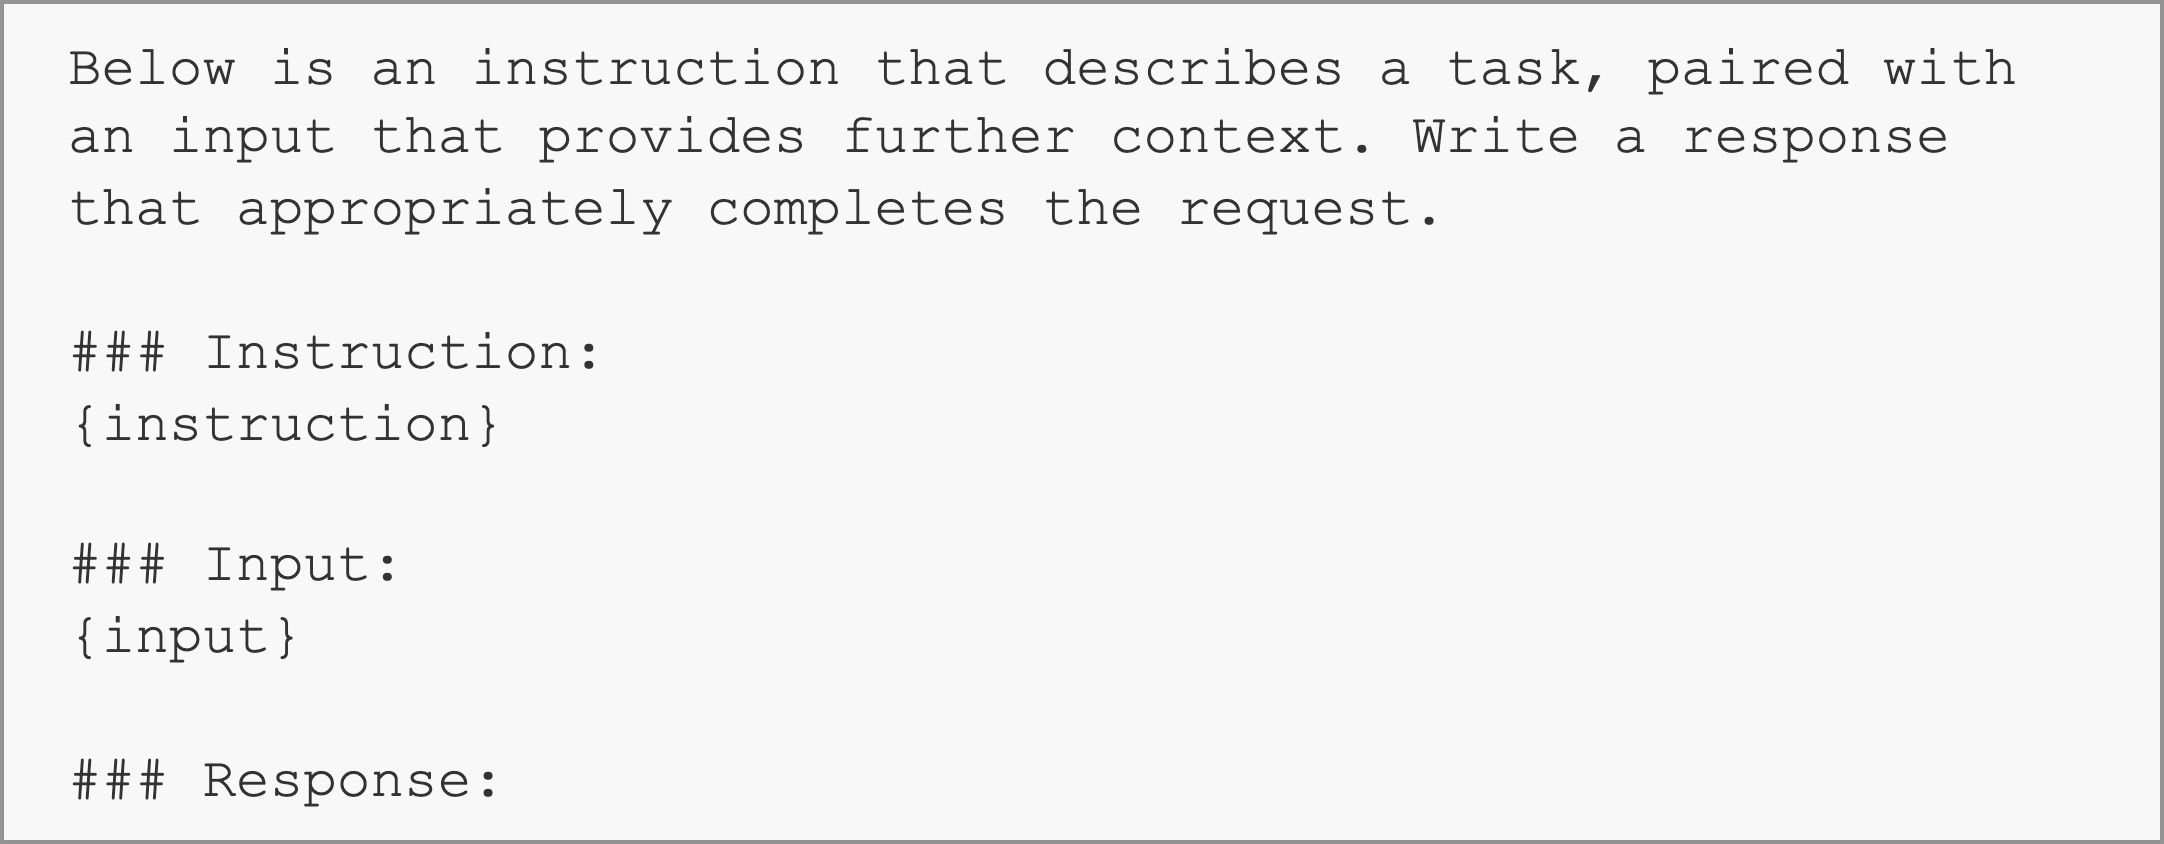
\includegraphics[width=\textwidth]{images/alpaca_prompt_format.png}}
            \caption[Overview of the original text prompt to the Stanford Alpaca model, with additional input.]{Overview of the original text prompt to the Stanford Alpaca model \cite{taoriStanfordCRFM, taoriStanfordAlpacaInstructionfollowing2023}, with additional input.}
            \label{fig:alpaca_prompt_format}
        \end{figure}

        % Modified prompt format
        \begin{figure}[htb]
            \centerline{
            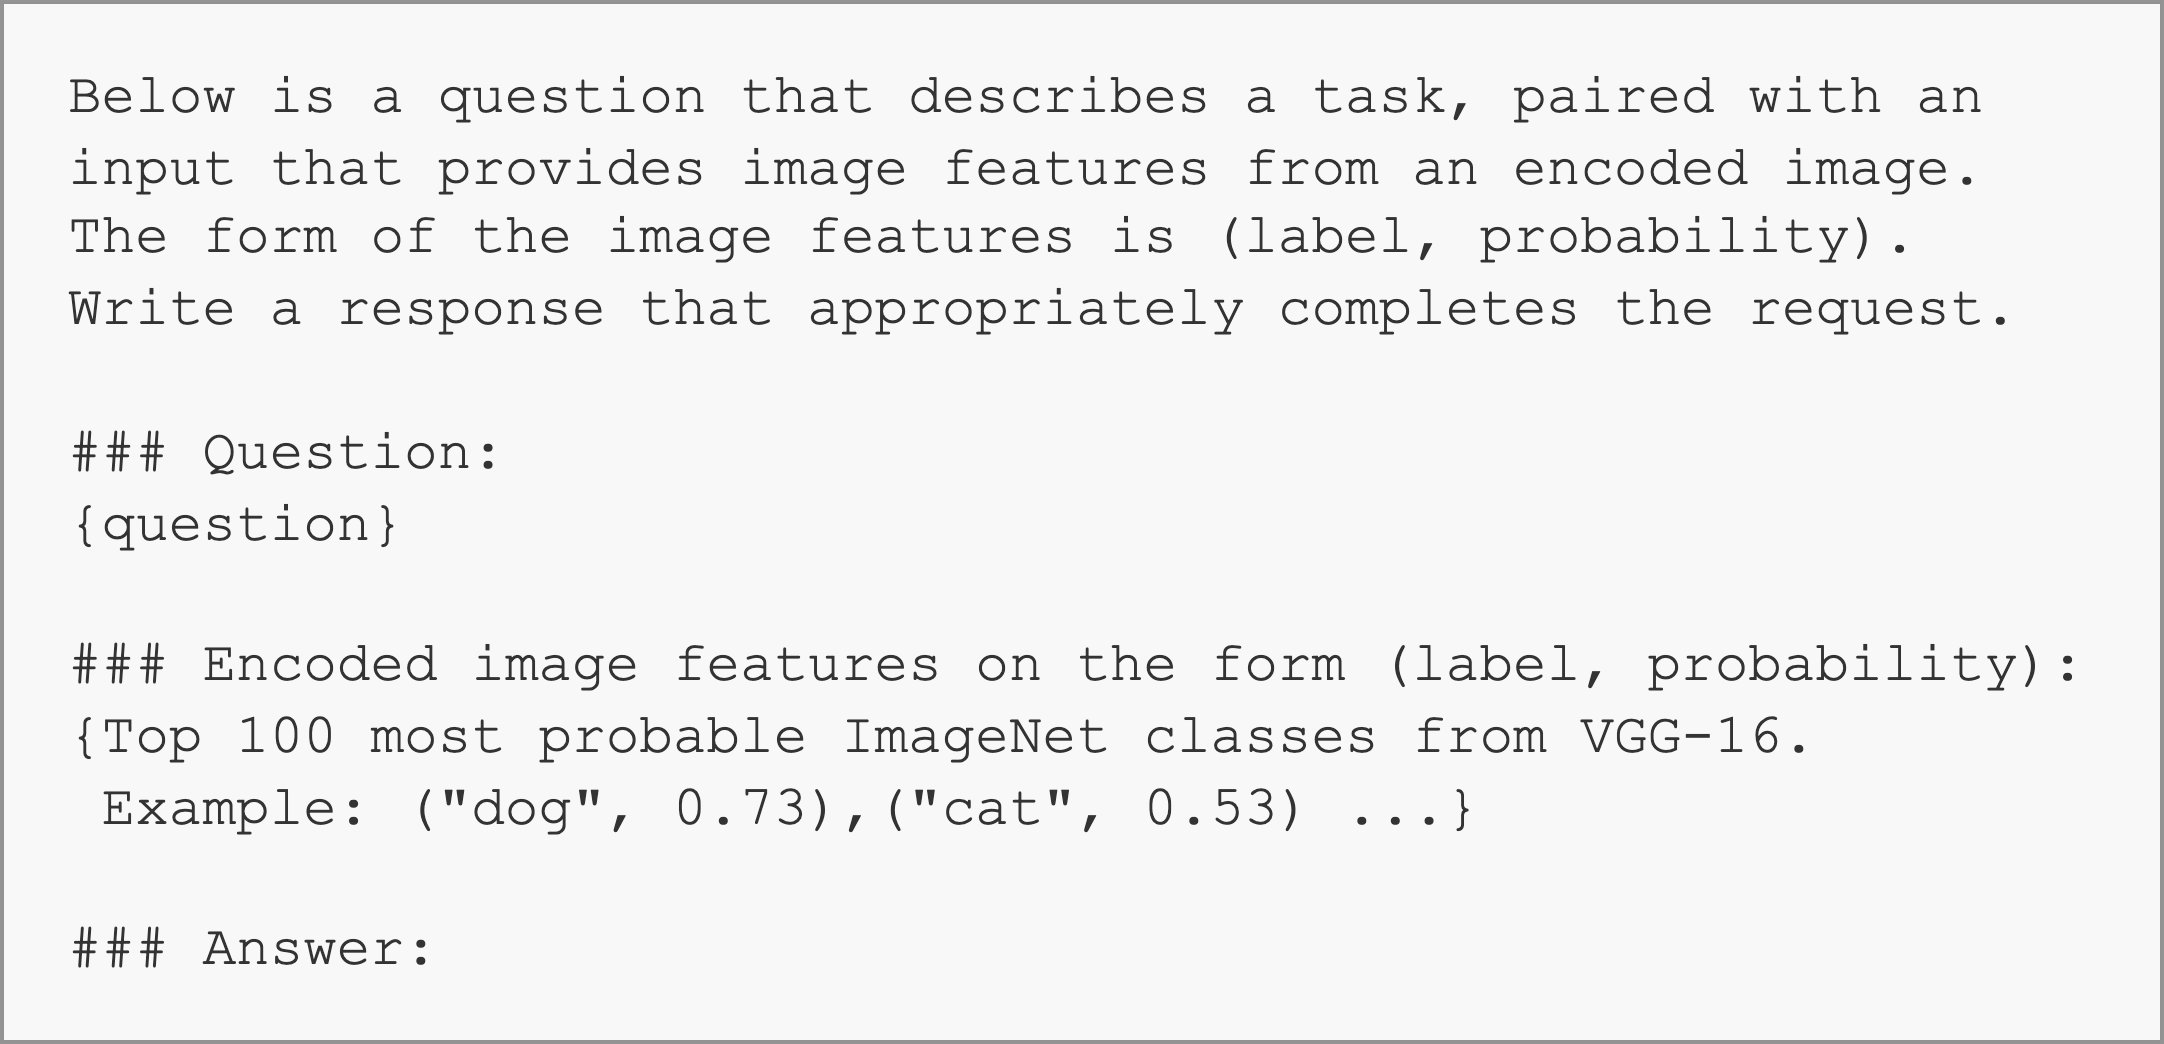
\includegraphics[width=\textwidth]{images/alpaca_modified_prompt_format.png}}
            \caption{Overview of the modified text prompt to the Alpaca-LoRA model, including extracted image features.}
            \label{fig:alpaca_modified_prompt_format}
        \end{figure}


        \subsubsection{Text encoding}
        \label{sec2:text_encoding}
        % How to encode the text

        A text tokenization process is needed to break down the raw text data given in the prompt into smaller, standardized units called tokens. This assures that text models, \glspl{llm} in this case, tokenization is essential to transform unstructured text data into a format that the model can process.
        
        Given that \glspl{llm} have been trained on specific tokenization schemes that use unique tokenization rules and vocabularies. If a different tokenizer is used to pre-process the text data, the tokenization output may not be compatible with the language model's vocabulary and encoding scheme, leading to poor model performance and incorrect predictions.
        
        Using the tokenizer from the language model ensures that the tokenization process is consistent with the training data and the model's internal encoding scheme. 
        
        This consistency ensures that the same tokenization scheme is used during both training and inference. This consistency is essential for the model to learn the patterns and relationships within the text data effectively. If a different tokenizer is used during inference, the output may not be the same as the input used during training, which in turn can lead to undesirable results.
        
        The tokenizer from the language model has also been trained on a large corpus of text data and optimized to handle specific language patterns and nuances. This makes it more effective than tokenization schemes that may not have the same optimization and language-specific knowledge level. Using the language model's tokenizer ensures that the text data is pre-processed in a way that is most compatible with the model, leading to better performance and more accurate predictions.

        The tokenizer used in this implementation is the one used by the original LLaMA model \cite{touvronLLaMAOpenEfficient2023}, and the specific implementation of the used LlamaTokenizer is based on SentencePiece \cite{LLaMATokenizer, Sentencepiece}. This tokenizer and detokenizer allow for an unsupervised, end-to-end system that does not need any language-specific processing. 

        % Datasets
    \subsection{}{Datasets}
    % ImageNet

    % MS COCO

    % Different VQA datasets
    
    % What is the VQA 2.0 dataset

     

        \subsubsection{Dataset Splitting}
        
        
    \subsection{Training the model}
        % How to train the model
        \subsubsection{Context window and cutoff length}
        \label{sec:3_cutoff}
        The context window of a language model refers to the number of words or tokens that are considered in predicting the next word or token. The context window is typically linked to both the input prompt and the output since the model refers to the input when generating the output. When training large language models, the model receives a sequence of input tokens and produces a sequence of output tokens. The context window refers to the size of the input sequence that the model uses to generate each output token. Similarly, when fine-tuning a pre-trained language model on a specific task, as in this case, the context window is also linked to both the input and the output. The input would consist of the task-specific prompt combined with the context window, and the output would be the predicted tokens that follow the input. By adjusting the size of the context window, researchers can control the amount of context that the model uses to generate its predictions, which can impact both the accuracy and the efficiency of the model.

        % how context window and cutoff length are related 
        Cutoff length is a term often used while fine-tuning a pre-trained language model for a specific task, where the model is fine-tuned on examples that consist of a prompt or query followed by a target output. The prompt cutoff length specifies the maximum length of the prompt that can be used during fine-tuning.

        The context window and cutoff length are, therefore, not the same, but closely related features that should be considered in conjunction with each other. In practice, the context window can therefore be seen as a way to capture longer-term dependencies between words in a sequence, while the prompt cutoff length is a constraint on the length of the input that the model is trained to handle for a specific task.
        
        

        % Specific cutoff length
        The updated input prompt shown in Figure \ref{fig:alpaca_modified_prompt_format} was used to training the model to interpret images. The prompt cutoff length was updated from the original 256 to 1485 tokens. The original LLaMA model was trained on 2048 tokens \cite{SequenceContextLength}, and the Alpaca model is fine-tuned with 512 tokens as the cutoff length. The authors of the Alpaca-LoRA model used in this experiment analyzed the training data and found that 96\% of the prompts could be answered by using a cutoff length of 256 tokens. When deciding on the new token length, including the top 100 classes from VGG-16, the LlamaTokenizer was used to encode only the features extracted from the image. 
        
        When the class prediction score was presented using Numpy's floating number with 32 bits of precision, the average token length only for image features where 162'654. As this would be an increase of the token length of more than 63 thousand percent, it was considered an increase too large to be reasonable for the model. Because the used language model uses the LoRA technique to lower memory consumption, such a large cutoff length would technically be feasible, but regarding the increased training and inference time, it was deemed too inefficient.  
        The prediction score was converted to floats with 16 bits of precision to decrease the image token length. In practice, this would not make a difference when fed into the language model, as the predicted class is just a placeholder for the underlying feature maps extracted. The upside of cutting the precision is that the average token length of the extracted 100 classes was cut down to 144'654 tokens. The reduced token length is an 11\% reduction of tokens, which still would benefit from a further reduction. To give a further decrease in the length of the prediction scores, they were rounded to three decimals. This will still give the language model insight into the extracted class labels and the relationship between the classes while also giving a great reduction in prediction score token length. The resulting rounded scores have a length of 1229 tokens, resulting in a reduction of 99\% from the original 32-bit precision score. Combined with a text prompt length of 256, the total cutoff length is 1485 tokens. This cutoff length is therefore designed to cover 96\% of the original prompts while also incorporating the 100 most probable classes and their predictions. 


         


        \subsubsection{Evaluation metrics}
        % Evaluation metrics used

       
        

        % Summary
        

% SUMMARY: